\documentclass[12pt]{article}
\usepackage[utf8]{inputenc}
\usepackage{amsmath}
\usepackage{amssymb}
\usepackage{graphicx}
\usepackage{comment}

\graphicspath{ {./plots/} }

\newcommand{\rectres}[1]{
\begin{center}
\begin{tabular}{ |c| }
\hline
\\
 #1\\
 \\
\hline
\end{tabular}
\end{center}
}

\newcommand{\qed}{\hfill$\blacksquare$}

\title{Introduction to Numerical Optimization\\Assignment 4}
%\author{Yair Nahum 034462796\\and\\blabla 11111111 }
\author{}

\begin{document}

\maketitle

%\tableofcontents{}

\section{Augmented Lagrangian method for Constrained Optimization}

\subsection{Graph}

We need to consider the following quadratic programming problem:
\begin{gather*}
    \min_{x_1,x_2}  2(x_1-5)^2 + (x_2-1)^2 \\
    \text{s.t \quad}\begin{array}{lr}
        x_2 \leq 1 - 0.5x_1 \\
        x_2 \geq x_1 \\
        x_2 \geq -x_1
    \end{array}
\end{gather*}
Which can be written as:
\begin{gather*}
    \min_{x_1,x_2}  2x^2_1-20x_1+50  + x^2_2-2x_2+1 \\
    \text{s.t \quad}\begin{array}{lr}
        0.5x_1 + x_2 -1 \leq 0  \\
        x_1- x_2 \leq 0 \\
        -x_1- x_2 \leq 0
    \end{array}
\end{gather*}
Or with matrices as:
\begin{gather*}
    \min_{x}  x^TAx + b^Tx + c \\
    \text{s.t \quad}\begin{array}{lr}
        Bx + d  \leq 0
    \end{array}
\end{gather*}
when:

\begin{itemize}
  \item $A \in \mathbb{R}^{2 \times 2}, A = \begin{bmatrix}
               2 & 0 \\
               0 & 1 \\
  \end{bmatrix}, x,b \in \mathbb{R}^{2}, b = \begin{bmatrix}   -20 \\ -2\\ \end{bmatrix}, c \in \mathbb{R}, c= 51$ 
  \item $B \in \mathbb{R}^{3 \times 2}, B = \begin{bmatrix}
               0.5 & 1 \\
               1 & -1 \\
               -1 & -1 \\
  \end{bmatrix}, d \in \mathbb{R}^{3}, d = \begin{bmatrix}   -1 \\ 0\\ 0\\\end{bmatrix}$
\end{itemize}

We plot the objective function contours (ellipses as we have different eigen values in our A matrix) and the constraints:\\
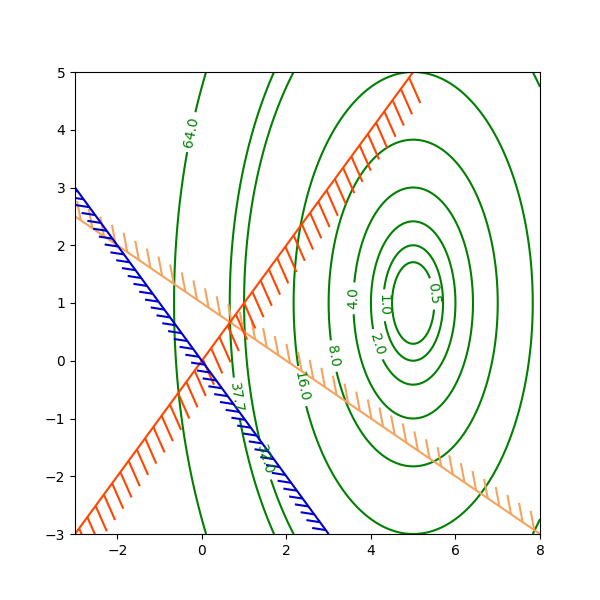
\includegraphics[scale=0.5]{hw4/plots/plot_1.png}\\
From plot, we can see the active constraints are the red and yellow together (the intersection point) and the blue ($-x_1- x_2 \leq 0$) is none active.\\
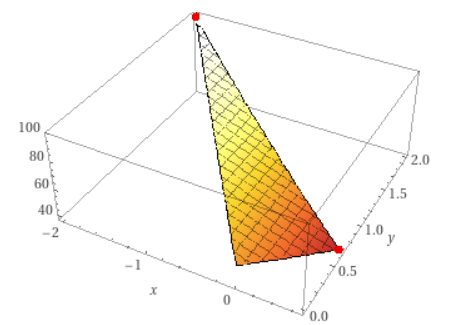
\includegraphics[scale=1]{hw4/plots/plot_2.png}\\

\subsection{Optimal Solution}

The intersection of the 2 active constraints when both are satisfied:
$$x_1=x_2, 0.5x_1+x_2=1 \Rightarrow x=(x_1,x_2)=(\frac{2}{3},\frac{2}{3}), f^*(x) = 37\frac{2}{3}$$

\subsection{KKT conditions}

The Lagrangian is defined as follows:
$$L(x,\lambda)=f(x) + \lambda^Tg(x) = f(x) + \Sigma_{i=1}^3\lambda_ig_i(x)$$

According to KKT, if $x^*$ is an optimal solution and $\nabla g_i(x)$ are independent (and we can see they are for any $x$ according to plot), we have $\lambda^* \in \mathbb{R}^3$ for which:\\
1. $\nabla_x L(x^*,\lambda^*) = 0$\\
2. $g(x^*)\leq0$\\
3. $\lambda_i^* \geq 0, i \in I_a$\\
4. $\lambda_i^* = 0, i \notin I_a$\\
$\Rightarrow$ And the complementary slackness:\\
5. $\Sigma_{i=1}^3\lambda_i^*g_i(x^*) = 0$\\

Note: since the constraints ($g_i(x)$) are affine functions then we stand with LCQ condition and no need for the independence condition for the above KKT first order conditions to hold.\\

Let's find the optimal point and multipliers:\\

1. $\nabla_x L(x^*,\lambda^*) = 0 \Rightarrow$\\
$$\nabla_{x_1} L(x^*,\lambda^*) = \nabla_{x_1} f(x^*) + \Sigma_{i=1}^3\lambda^*_i\nabla_{x_1} g_i(x^*) = 0\Rightarrow$$
$$\nabla_x_1 L(x^*,\lambda^*) = 4(x_1-5) + 0.5\lambda^*_1 + \lambda^*_2 -\lambda^*_3 = 0$$
$$\nabla_x_2 L(x^*,\lambda^*) = \nabla_{x_2} f(x^*) + \Sigma_{i=1}^3\lambda^*_i\nabla_{x_2} g_i(x^*) = 0\Rightarrow$$
$$\nabla_{x_2} L(x^*,\lambda^*) = 2(x_2-1) + \lambda^*_1 - \lambda^*_2 -\lambda^*_3 = 0$$

2. $g(x^*)\leq0$\\
$$ g_1(x^*) = 0.5x_1 +x_2 -1 \leq 0$$
$$ g_2(x^*) = x_1 -x_2 \leq 0$$
$$ g_3(x^*) = -x_1 -x_2 \leq 0$$

3. $\lambda_i^* \geq 0, i \in I_a$\\

4. $\lambda_i^* = 0, i \notin I_a$\\

5. $\Sigma_{i=1}^3\lambda_i^*g_i(x^*) = 0$\\
$$ \lambda_1^*g_1(x^*) = \lambda_1^*(0.5x_1 +x_2 -1) = 0$$
$$ \lambda_2^*g_2(x^*) = \lambda_2^*(x_1 -x_2) = 0$$
$$ \lambda_3^*g_3(x^*) = \lambda_3^*(-x_1 -x_2) = 0$$

From the last 2 equations of comp. slackness:\\
We have:\\
1. $x_1=x_2$ or $\lambda_2^*=0$\\
2. $x_1=-x_2$ or $\lambda_3^*=0$\\

If we assume $x_1=x_2 = -x_2$ we get the optimal point is $x_1=x_2=0 \Rightarrow \lambda^*_1 = 0, \lambda^*_3 = \frac{-22}{2}=-11<0$ (from $\lambda_1^*(0.5x_1 +x_2 -1) = 0$ and $\nabla_x L(x^*,\lambda^*) = 0$), and we get a contradiction.\\

So, $x_1=x_2,\lambda^*_3=0$ or $x_1=-x_2,\lambda^*_2=0$\\

if $x_1=-x_2,\lambda^*_2=0$\\
From $$\lambda_1^*(0.5x_1 +x_2 -1) = 0\Rightarrow$$
$$\lambda_1^*(-0.5x_1 -1) = 0$$
We get $\lambda_1^*=0$ or $x_1=-2, x_2=2$\\

if $x_1=-2, x_2=2$\\
from first equations we get:\\
$$4(x_1-5) + 0.5\lambda^*_1 -\lambda^*_3 = 0$$
$$2(-x_1-1) + \lambda^*_1 -\lambda^*_3 = 0 \Rightarrow$$
$$6x_1-18 - 0.5\lambda^*_1 = 0\Rightarrow$$
$\lambda^*_1<0$ and we get a contradiction again as $\lambda^*_1\geq 0$\\

if $\lambda^*_1=0$\\
from first equations we get:\\
$$4(x_1-5) -\lambda^*_3 = 0$$
$$2(-x_1-1) -\lambda^*_3 = 0 \Rightarrow$$
$$x_1=3, \lambda^*_3 <0$$ and again we get a contradiction as $\lambda^*_3\geq 0$\\

Thus, we are left with:\\
$$x_1=x_2,\lambda^*_3=0$$
From $$\lambda^*_1(0.5x_1 +x_2 -1) = 0\Rightarrow$$
$$\lambda^*_1(1.5x_1 -1) = 0$$
We get $\lambda^*_1=0$ or $x_1=\frac{2}{3}, x_2=\frac{2}{3}$\\

if $\lambda^*_1=0$\\
from first equations we get:\\
$$4(x_1-5) +\lambda^*_2 = 0$$
$$2(x_1-1) -\lambda^*_2 = 0 \Rightarrow$$
$$x_1=\frac{22}{6}, \lambda^*_2 = \frac{16}{3}$$

But in this case we get a contradiction from:
$$ g_1(x^*) = 0.5x_1 +x_2 -1 \leq 0$$\\

Bottom line, we are left with:\\
$$x_1=x_2=\frac{2}{3},\lambda^*_3=0$$

From first equations we get:\\
$$4(x_1-5)  + 0.5\lambda^*_1 +\lambda^*_2 = 0$$
$$2(x_1-1)  + \lambda^*_1 -\lambda^*_2 = 0 \Rightarrow$$
$$\frac{-52}{3}  + 0.5\lambda^*_1 +\lambda^*_2 = 0$$
$$-\frac{2}{3}  + \lambda^*_1 -\lambda^*_2 = 0 \Rightarrow$$
$$\frac{3}{2}\lambda^*_1 = \frac{54}{3} = 18 \Rightarrow$$
\rectres{$\lambda^*_1 = 12,\lambda^*_2 = 11\frac{1}{3}, \lambda^*_3=0$}

\subsection{Dual Problem}

Since we have KKT conditions with a convex problem (convex objective function, convex constraints (even linear in our case)), then strong duality holds. Meaning:\\
$$f^*(x^*,\lambda^*) = min_x \{max_{\lambda \geq 0} L(x,\lambda)\} =  max_{\lambda \geq 0}\{min_x L(x,\lambda)\}$$

Let's define the dual function $\eta(\lambda) = min_x L(x,\lambda)$:\\

First we find $x^*$ by taking the derivative of the Lagrangian and comparing it to 0. This is enough for finding the optimal point as the Lagrangian is a convex function.\\

The Lagrangian:
\begin{gather*}
    L(x,\lambda) =  x^TAx + b^Tx + c + \lambda^T (Bx + d)\\
\end{gather*}

When:\\

\begin{itemize}
  \item $A \in \mathbb{R}^{2 \times 2}, A = \begin{bmatrix}
               2 & 0 \\
               0 & 1 \\
  \end{bmatrix}, x,b \in \mathbb{R}^{2}, b = \begin{bmatrix}   -20 \\ -2\\ \end{bmatrix}, c \in \mathbb{R}, c= 51$ 
  \item $B \in \mathbb{R}^{3 \times 2}, B = \begin{bmatrix}
               0.5 & 1 \\
               1 & -1 \\
               -1 & -1 \\
  \end{bmatrix}, d \in \mathbb{R}^{3}, d = \begin{bmatrix}   -1 \\ 0\\ 0\\\end{bmatrix}$
\end{itemize}

Therefore:\\

$$\nabla_x L(x,\lambda) = 2Ax + b + B^T\lambda = 0 \Rightarrow$$
$$ x^* = -\frac{1}{2}A^{-1}(B^T\lambda + b)$$


We next put it in the Lagrangian to get the dual function:\\
Note: A is diagonal in our case so it's also symmetric (and its inverse as well).\\

$$\eta(\lambda) = L(x^*,\lambda) = \frac{1}{4}(B^T\lambda + b)^TA^{-1}(B^T\lambda + b) -\frac{1}{2}b^TA^{-1}(B^T\lambda + b) + \lambda^T (-\frac{1}{2}BA^{-1}(B^T\lambda + b) + d)=$$
$$=\frac{1}{4}\lambda^TBA^{-1}B^T\lambda+\frac{1}{2}b^TA^{-1}B^T\lambda+\frac{1}{4}b^TA^{-1}b-\frac{1}{2}b^TA^{-1}B^T\lambda-\frac{1}{2}b^TA^{-1}b-\frac{1}{2}\lambda^TBA^{-1}B^T\lambda$$
$$-\frac{1}{2}\lambda^TBA^{-1}b + \lambda^Td=$$
$$=-\frac{1}{4}\lambda^TBA^{-1}B^T\lambda -\frac{1}{2}\lambda^TBA^{-1}b-\frac{1}{4}b^TA^{-1}b + \lambda^Td $$

As expected, this is a concave function in $\lambda$

So, the dual problem is:
\rectres{$\max_{\lambda \geq 0} \eta(\lambda)=\max_{\lambda \geq 0}-\frac{1}{4}\lambda^TBA^{-1}B^T\lambda -\frac{1}{2}\lambda^TBA^{-1}b-\frac{1}{4}b^TA^{-1}b + \lambda^Td$}

When:\\
\begin{itemize}
  \item $A \in \mathbb{R}^{2 \times 2}, A = \begin{bmatrix}
               2 & 0 \\
               0 & 1 \\
  \end{bmatrix}, x,b \in \mathbb{R}^{2}, b = \begin{bmatrix}   -20 \\ -2\\ \end{bmatrix}, c \in \mathbb{R}, c= 101$ 
  \item $B \in \mathbb{R}^{3 \times 2}, B = \begin{bmatrix}
               0.5 & 1 \\
               1 & -1 \\
               -1 & -1 \\
  \end{bmatrix}, d \in \mathbb{R}^{3}, d = \begin{bmatrix}   -1 \\ 0\\ 0\\\end{bmatrix}$
\end{itemize}

\subsection{Dual Optimum}

Let's check that optimal $x^*$ is achieved when setting the optimal multipliers:

$$ x^* = -\frac{1}{2}A^{-1}(B^T\lambda + b)$$
When:\\
$ \lambda^* = \begin{bmatrix} 
    12 \\
    11\frac{1}{3}\\
    0\\
    \end{bmatrix}
  A^{-1} = \begin{bmatrix}
               \frac{1}{2} & 0 \\
               0 & 1 \\
  \end{bmatrix},
  B^T = \begin{bmatrix}
               0.5 & 1 & -1\\
               1 & -1 & -1\\
  \end{bmatrix},
  b = \begin{bmatrix}   -20 \\ -2\\ \end{bmatrix}$\\
Therefore:\\
$$ x^* = -\frac{1}{2}A^{-1}(B^T\lambda + b)=-\frac{1}{2}
  \begin{bmatrix}
               \frac{1}{2} & 0 \\
               0 & 1 \\
  \end{bmatrix}(
  \begin{bmatrix}
               0.5 & 1 & -1\\
               1 & -1 & -1\\
  \end{bmatrix}
  \begin{bmatrix} 
    12 \\
    \frac{34}{3}\\
    0\\
  \end{bmatrix}
    +
  \begin{bmatrix}   -20 \\ -2\\ \end{bmatrix})    
  =$$
  $$=-\frac{1}{2}
  \begin{bmatrix}
               \frac{1}{2} & 0 \\
               0 & 1 \\
  \end{bmatrix}(\begin{bmatrix} \frac{52}{3} \\ \frac{2}{3}\\ \end{bmatrix} + \begin{bmatrix}   -20 \\ -2\\ \end{bmatrix})=$$
  $$=-\frac{1}{2}
  \begin{bmatrix}
               \frac{1}{2} & 0 \\
               0 & 1 \\
  \end{bmatrix}\begin{bmatrix}   -\frac{8}{3} \\ -\frac{4}{3}\\ \end{bmatrix}=$$
$$=\begin{bmatrix} \frac{2}{3} & \frac{2}{3}\\ \end{bmatrix}^T \Rightarrow$$

\rectres{$x^*=\begin{bmatrix} \frac{2}{3} & \frac{2}{3}\\ \end{bmatrix}^T$}

Exactly like we got at the primal problem solution. So we conclude that the dual optimum is achieved at that point as expected due to strong duality in this case.

\subsection{Augmented Lagrangian Solver}
In code.\\
We've defined 3 main classes:\\
1. OptimizationProblem - objective functions pointers' to value,gradient and hessian + the same for constraints functions (w/ or w/o constraints)\\
2. Penalty - manages the penalty function value and derivatives calculations + considers penalty parameter and multiplier\\
3. AugmentedLagarangianSolver - the main class\\

Note: we've limited the multipliers increase/decrease relative to previous multiplier by factor of 3 (as suggested in lectures).

\subsection{Testing solver}
Some snippets from code outputs:\\
Newton Method has converged after 6 iterations\\
Newton Method has converged after 6 iterations\\
Newton Method has converged after 7 iterations\\
Newton Method has converged after 6 iterations\\

We can see the x values have converged to the optimal x under constraints as calculates:\\
x\_traj=array([[ 0. ], [-0.2]]),\\ array([[0.09900358],
       [0.02088282]]), array([[0.82696752],
       [0.75244632]]), array([[0.80335486],
       [0.70356693]]), array([[0.80387324],
       [0.70393907]]), array([[0.80386339],
       [0.70393477]]), array([[0.80386357],
       [0.70393483]]), array([[ 0. ],
       [-0.2]]), array([[0.04311619],
       [0.01379573]]), array([[0.64303387],
       [0.61516818]]), array([[0.71960123],
       [0.69190039]]), array([[0.72342876],
       [0.6824236 ]]), array([[0.72340545],
       [0.68244142]]), array([[0.72340564],
       [0.68244143]]), array([[ 0. ],
       [-0.2]]), array([[0.01385387],
       [0.01412047]]), array([[0.45665664],
       [0.45744669]]), array([[0.65601656],
       [0.65706519]]), array([[0.67112535],
       [0.67215757]]), array([[0.67549307],
       [0.66969653]]), array([[0.6754751 ],
       [0.66969512]]), array([[0.67547518],
       [0.66969514]]), array([[ 0. ],
       [-0.2]]), array([[0.00544623],
       [0.00846268]]), array([[0.61151288],
       [0.5594119 ]]), array([[0.70594954],
       [0.65477842]]), array([[0.66662328],
       [0.66666689]]), array([[0.66670718],
       [0.66668043]]),\\
       \textbf{array([[0.66670699],[0.66668037]])}\\

We can also see the multipliers have converged close to thier optimal calculated values:\\
multipliers=\\
array([[1.],[1.],[1.]]),\\
       array([[3.        ],
       [3.        ],
       [0.33333333]]),\\
       array([[9.        ],
       [9.        ],
       [0.11111111]]),\\
       \textbf{array([[11.97309228],
       [11.31201791],
       [ 0.03703704]])}
       
\subsection{Plots}
\subsubsection{}
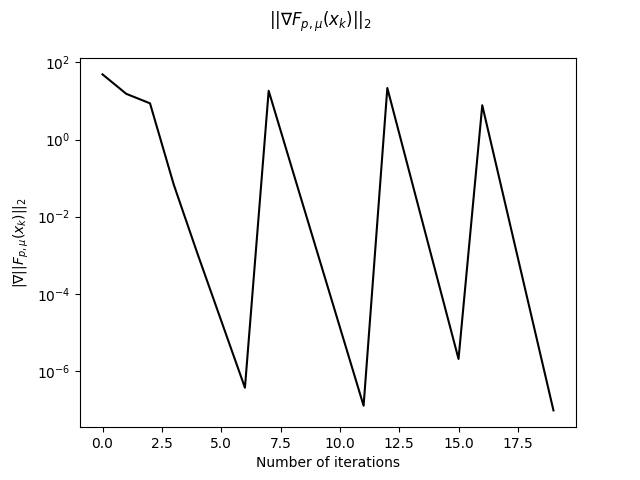
\includegraphics[scale=0.5]{hw4/plots/plot_3.png}\\
We can see in above plot that the gradients on each newton iteration converged in a polynomial convergence rate. In between, we ruin our current point a bit as we change the penalty parameter (increase by $\alpha=2$) and multipliers (derivative at active points).\\

\subsubsection{}
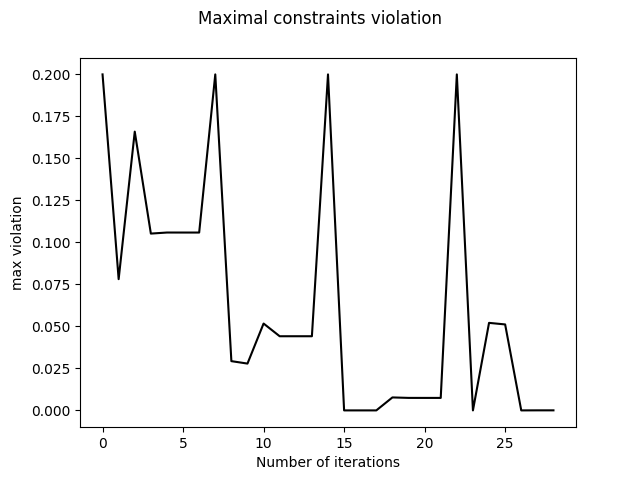
\includegraphics[scale=0.5]{hw4/plots/plot_4.png}\\
Above is the plot of the maximum constraint violation $\max_i(g_i(x)) \geq 0$ at each x in the trajectory we've followed.\\

\subsubsection{}
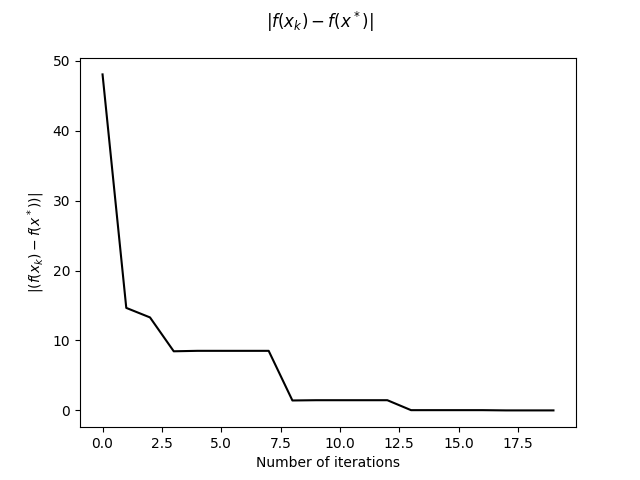
\includegraphics[scale=0.5]{hw4/plots/plot_5.png}\\
The absolute value of the diff between the x trajectory function's values and the optimal x function value (for the constrained problem). we can see we eventually converge to the optimal value (diff is zero)\\

\subsubsection{}
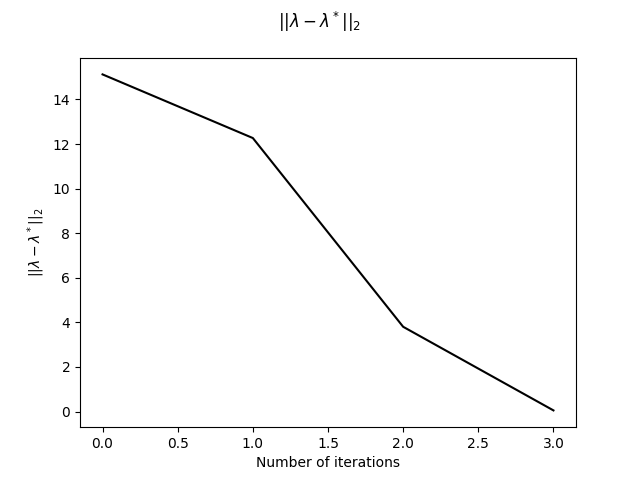
\includegraphics[scale=0.5]{hw4/plots/plot_6.png}\\
We can see the distance between trajectory x values and optimal x converges to 0. The same bumps as we saw due to restating a new unconstrained optimization problem with different penalty and multipliers.\\
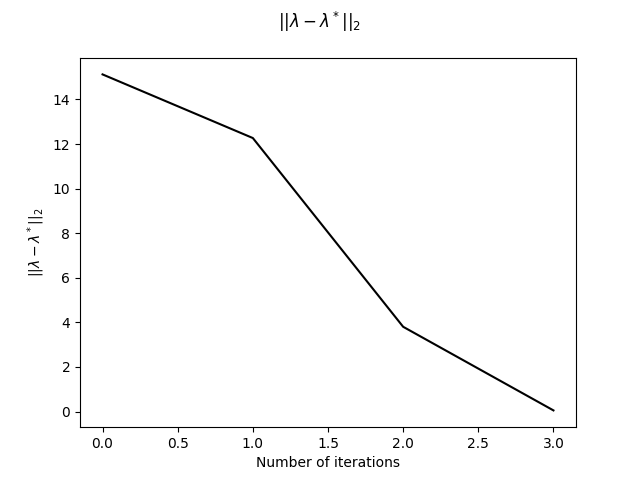
\includegraphics[scale=0.5]{hw4/plots/plot_7.png}\\
On multipliers, we can see we converge to the optimal monotonically as we update them between new unconstrained optimization problems (defined on new penalty function aggregate)\\

\begin{comment}

\section{Constrained Optimization and Duality}

\subsection{Question 1}
We need to solve the following 
\begin{equation}
\label{eq:min1}
\begin{split}
    \min _x x^T M x + c^T x \\
    \text{s.t. } Ax = b
\end{split}
\end{equation}
Given:
\begin{itemize}
  \item $M \in \mathbb{R}^{n\times n},M \succ 0$
  \item $A \in \mathbb{R}^{m\times n}$
  \item $x,c \in \mathbb{R}^{n}$
  \item $b \in \mathbb{R}^{m}$
  \item Assuming $M$ and $AM^{-1}A^T$ are invertible.
\end{itemize}
M is P.D $\Rightarrow$ it is Hermitian ($M=M^*$), and since $M \in \mathbb{R}^{n\times n}$ it is symmetric($M=M^T$).\\
We require the KKT conditions (necessary conditions for $x^*$ to be optimal).\\
These conditions hold as this is a convex problem with only linear constraints.
The Lagrangian is:
$$L(x,\mu)=x^T M x + c^T x + \mu^T(Ax-b)$$
The first KKT condition $\nabla_x L(x,\mu)=0$:
$$\nabla_x L(x,\mu)=0 = 2Mx + c + A^T\mu \Rightarrow$$
$$x^* = -\frac{1}{2}M^{-1}(c + A^T\mu^*)$$
The $M$ is invertible since it is P.D.\\
The third KKT condition gives $h_i(x)=Ax-b=0$, if we put the $x^*$ in it we can isolate and get $\mu^*$:\\
$$-\frac{1}{2}AM^{-1}(c + A^T\mu^*) = b \Rightarrow$$
$$b+\frac{1}{2}AM^{-1}c = -\frac{1}{2}AM^{-1}A^T\mu^* \Rightarrow$$
$$\mu^* = -(AM^{-1}A^T)^{-1}(2b+AM^{-1}c)$$
We put back in $x^*$ :\\
$$x^* = -\frac{1}{2}M^{-1}(c + A^T\mu) =-\frac{1}{2}M^{-1}(c + A^T(-(AM^{-1}A^T)^{-1}(2b+AM^{-1}c))) \Rightarrow $$
\rectres{$$x^* =  \frac{1}{2}M^{-1}(A^T(AM^{-1}A^T)^{-1}(2b+AM^{-1}c)-c)$$}
\newpage
\subsection{Question 2}

We need to solve the following 
\begin{equation}
\label{eq:min2}
\begin{split}
    \min _x ||x - c||^2_2 \\
    \text{s.t. } Ax = b
\end{split}
\end{equation}
Given:
\begin{itemize}
  \item $A \in \mathbb{R}^{m\times n}$
  \item $x,c \in \mathbb{R}^{n}$
  \item $b \in \mathbb{R}^{m}$
  \item Assuming $AA^T$ is invertible.
\end{itemize}

We require the KKT conditions (necessary conditions for $x^*$ to be optimal).\\
These conditions hold as this is a convex problem with only linear constraints.
The Lagrangian is:
$$L(x,\mu)=x^Tx -2c^T x + c^Tc + \mu^T(Ax-b)$$
The first KKT condition $\nabla_x L(x,\mu)=0$:
$$\nabla_x L(x,\mu)= 0 = 2x -2c + A^T\mu \Rightarrow$$
$$x^* = (c - \frac{1}{2} A^T\mu^*)$$
The third KKT condition gives $h_i(x)=Ax-b=0$, if we put the $x^*$ in it we can isolate and get $\mu^*$:\\
$$b = A(c - \frac{1}{2} A^T\mu) \Rightarrow$$
$$\mu^* = 2(AA^T)^{-1}(Ac-b)$$
We put back in $x^*$ :\\
$$x^* = c - \frac{1}{2} A^T\mu^* = c - \frac{1}{2} A^T (2(AA^T)^{-1}(Ac-b))  \Rightarrow  $$
\rectres{$$x^* =   c - A^T(AA^T)^{-1}(Ac-b)$$}

\newpage

\subsection{Question 3}

\begin{equation}
\label{eq:min3}
\begin{split}
    \min _x x^T A x + b^T x \\
    \text{s.t. } \\
    1^T_3x = 1\\
    x_3 \leq 1\\
\end{split}
\end{equation}
Given:
\begin{itemize}
  \item $A \in \mathbb{R}^{3 \times 3}$
  \item $x,b,1_3 \in \mathbb{R}^{3}$
  \item $A = \begin{bmatrix}
               1 & 1 & 0 \\
                1 & 2 & 0 \\
                0 & 0 & 0 \\
              \end{bmatrix}$
  \item $b = \begin{bmatrix}  1 \\ -1 \\ 1\\ \end{bmatrix}$
  \item $1_3 = \begin{bmatrix} 1\\  1\\  1\\ \end{bmatrix}$
\end{itemize}

\subsubsection{Is the problem convex?}
Since the constraints functions are linear $g_i(x),h_i(x)$ they are also convex.\\
The target function is convex iff $A\succcurlyeq 0$.
To check this, we can check all the principal minors to be $M_{i,i}\geq 0$ or by finding all eigenvalues to be $\lambda_i \geq 0$. 
\begin{itemize}
  \item There are 7 principal minors for $3\times3$ matrix $m=2^n-1$. The minors are: 1 ,2 ,0, 0, 0 ,1 ,0. so we found that all are greater or equal to 0. Therefore, $A\succcurlyeq 0$.
  \item Finding the eigenvalues by $det(\lambda I - A) = 0 \Rightarrow$:\\
  $$0=\lambda((\lambda-2)(\lambda-1)-1)=\lambda(\lambda^2-3\lambda+1)\Rightarrow$$
  $$\lambda_1=0, \lambda_{2,3}=\frac{3\pm \sqrt{5}}{2} \Rightarrow$$
  All eigenvalues are greater or equal to 0. Therefore, $A\succcurlyeq 0$.
\end{itemize}
Bottom line, the problem is convex as $A$ is positive semi definite. 
\subsubsection{Find and solve the dual problem}
Since the problem is convex and the constraints are linear, the Slater's condition (SC) holds and the strong duality is valid.\\
Let's first define the primal problem.\\
The constraints:\\
$$g_1(x)=\begin{bmatrix}  0 & 0 & 1 \end{bmatrix}^T x - 1\leq 0$$
$$h_1(x)=1^T_3 x - 1 = 0$$
The Lagrangian is as follows:\\
$$L(x,\mu,\lambda)=x^T A x + b^T x + \mu_1 h_1(x) + \lambda_1 g_1(x)$$
The primal problem is therefore:
$$p* = \min _x \max _{\mu,\lambda \geq 0} L(x,\mu,\lambda)$$
The dual function is:
$$\eta(\mu,\lambda) = \min _x L(x,\mu,\lambda) $$
The dual problem is therefore:
$$d* =  \max _{\mu,\lambda \geq 0} \min _x L(x,\mu,\lambda) = \max _{\mu,\lambda \geq 0} \eta(\mu,\lambda)$$
The KKT conditions hold. Let's solve the dual problem.\\
We can find $\eta(\mu,\lambda) = \min _x L(x,\mu,\lambda)$ (the optimal $x^*$ for specific $\mu,\lambda$) by the KKT condition $\nabla_x L(x,\mu,\lambda) = 0$:
$$\nabla_x L(x,\mu,\lambda) = 2Ax + b + \mu_1 1_3 + \lambda_1 \begin{bmatrix}  0 \\ 0 \\ 1 \end{bmatrix} = 0 \Rightarrow$$
$$ 2 \begin{bmatrix} 1 & 1 & 0 \\ 1 & 2 & 0 \\ 0 & 0 & 0 \\ \end{bmatrix} x + 
\begin{bmatrix}  \mu_1 + 1 \\ \mu_1 - 1 \\ \mu_1 + \lambda_1 + 1\\ \end{bmatrix} = 0 \Rightarrow$$
We get 3 equations:\\
\setcounter{equation}{0}
\begin{equation}
2x_1 + 2x_2 +\mu_1 + 1 = 0
\end{equation}
\begin{equation}
2x_1 + 4x_2 +\mu_1 - 1 = 0
\end{equation}
\begin{equation}
\mu_1 + \lambda_1 + 1 = 0
\end{equation}
By subtracting equations (2) - (1) we get $x_2$:
$$2x_2 = 2 \Rightarrow x_2 = 1$$
Therefore, $x_1$:
$$x_1 = -\frac{1}{2}(\mu_1+3)$$
From the third KKT condition (the constraints) we get:
$$1_3^T x = 1 \Rightarrow$$
$$x_3 = -x_1 = \frac{1}{2}(\mu_1+3)$$
So, we got the following expression for $x*$:
$$x^* = \begin{bmatrix}  -\frac{1}{2}(\mu_1+3) \\ 1 \\ \frac{1}{2}(\mu_1+3) \end{bmatrix}$$
Providing the constraint:
$$\mu_1 + \lambda_1 + 1 = 0$$
Setting the $x^*$ in the Lagrangian, we get the dual function:
$$\eta(\mu,\lambda) = \min _x L(x,\mu,\lambda) = L(x^*,\mu,\lambda) = x^{*T} A x^* + b^T x^* + \mu_1 (1_3^T x^* - 1) + \lambda_1 (x^*_3-1)$$
$$x^{*T} A x^* = \begin{bmatrix}  x^*_1 & x^*_2 & x^*_3 \end{bmatrix} 
\begin{bmatrix} 1 & 1 & 0 \\ 1 & 2 & 0 \\ 0 & 0 & 0 \\ \end{bmatrix} 
\begin{bmatrix}  x^*_1 \\ x^*_2 \\ x^*_3 \end{bmatrix} = $$
$$\begin{bmatrix} x^*_1+1  & x^*_1+2 & 0 \end{bmatrix}
\begin{bmatrix}  x^*_1 \\ 1 \\ x^*_3 \end{bmatrix}
 =x^*_1^2 + 2x^*_1 + 2$$
$$ b^T x^* = \begin{bmatrix}  1 & -1 & 1 \end{bmatrix} \begin{bmatrix}  x^*_1 \\ 1 \\ -x^*_1 \end{bmatrix} = -1$$
Combining it together we get the dual function after minimizing by x:
$$\eta(\mu,\lambda) =  L(x^*,\mu,\lambda) = x^*_1^2 + 2x^*_1 + 2 - 1 + \lambda_1 (x^*_3-1) = x^*_1^2 + (2-\lambda_1) x^*_1 + 1 - \lambda_1  =$$
$$\frac{1}{4}(\mu_1 + 3)^2 + (\lambda_1-2) (\frac{1}{2}(\mu_1+3) + 1 - \lambda_1$$

The dual problem is therefore:
\rectres{
$$d^* =  \max _{\mu_1,\lambda_1} [ \frac{1}{4}(\mu_1 + 3)^2 + (\lambda_1-2) (\frac{1}{2}(\mu_1+3) + 1 - \lambda_1 ] \\ \text{s.t. } \mu_1 + \lambda_1 + 1 = 0, \lambda_1 \geq 0$$
}
Solving the dual problem, we use the linear constraint (part of KKT conditions that the constraint holds) $ \lambda_1 = - \mu_1 - 1$ and put it in the target function:
$$\eta(\mu,\lambda) = [ \frac{1}{4}(\mu_1 + 3)^2 + (\lambda_1-2) (\frac{1}{2}(\mu_1+3) + 1 - \lambda_1 ] = [ \frac{1}{4}(\mu_1 + 3)^2 - (\mu_1+3) (\frac{1}{2}(\mu_1+3) + 2 + \mu_1 ] = $$ $$\frac{\mu_1^2+6\mu + 9}{4} - \frac{\mu_1^2+6\mu_1 + 9}{2} + 2 + \mu_1 = - \frac{\mu_1^2+6\mu_1 + 9}{4} + 2 + \mu_1 =  \frac{-\mu_1^2 -6\mu_1 - 9 + 8 + 4\mu_1}{4}=$$
$$\frac{-\mu_1^2 -2\mu_1 - 1}{4}$$
We can see that this is a concave function, therefore it has a maximum.\\
Calculating the derivative and compare to 0 we get:
$$\eta'(\mu_1) = \frac{-\mu_1 -1}{2} = 0 \Rightarrow$$
$$\mu_1^* = -1$$
And by the constraint:
$$\lambda^*_1 = 0$$
Putting it back in $x*$ we get:\\
$$x^* = \begin{bmatrix}  -\frac{1}{2}(\mu_1+3) \\ 1 \\ \frac{1}{2}(\mu_1+3) \end{bmatrix} = \begin{bmatrix}  -1 \\ 1 \\ 1 \end{bmatrix}$$
And the function minimum value:
$$f*=p*=d*=\frac{-\mu_1^2 -2\mu_1 - 1}{4} = 0$$
\rectres{
$$x^* = \begin{bmatrix}  -1 \\ 1 \\ 1 \end{bmatrix}, f* = 0$$
}
\newpage
\subsection{Question 4}
We need to find and write the dual problem of the following linear programming problem:
\setcounter{equation}{0}
\begin{equation}
\label{eq:min4}
\begin{split}
    \min _x c^T x \\
    \text{s.t. }\\
    Ax \leq b\\
    x \geq 0
\end{split}
\end{equation}
Given:
\begin{itemize}
  \item $A \in \mathbb{R}^{m\times n}$
  \item $x,c \in \mathbb{R}^{n}$
  \item $b \in \mathbb{R}^{m}$
\end{itemize}
First we will define the primal problem:
$$p^*=\min_x \max_{\mu,\lambda \geq 0} L(x,y,\lambda)$$
When the Lagrangian is:
$$L(x,y,\lambda) = c^T x + y^T (Ax-b) -\lambda^T x$$
$$\\y,\lambda \in \mathbb{R}^m$$

The problem is convex with linear only constraints, so by Slater's condition we have strong duality.\\
That is:
$$p^*=\min_x \max_{y \geq 0,\lambda \geq 0} L(x,y,\lambda) = \max_{y \geq 0,\lambda \geq 0} \min_x  L(x,y,\lambda) = d^*$$
The dual function $\eta(y,\lambda)$ is:
$$\eta(y,\lambda) = \min_x  L(x,y,\lambda)$$
To find the dual problem, we will compare the $\nabla_x (x,y,\lambda)$ to zero according to KKT conditions:\\
$$\nabla_x (x,y,\lambda) = c + A^Ty - \lambda = 0$$
This means that the dual problem has a constraint:\\
$$c = \lambda-A^Ty $$
From complementary slackness $y^T (Ax-b) -\lambda^T x= 0 \Rightarrow$:
$$(y^T A - \lambda^T)x - y^Tb = 0 \Rightarrow $$
$$-c^Tx - y^Tb = 0 \Rightarrow c^Tx = - y^Tb$$
And therefore the Lagrangian doesn't depend on x:\\
$$L(x,y,\lambda) = - y^Tb$$
(BTW, we can also get the Lagrangian by just setting $c=\lambda -A^Ty$)\\
So, the dual function is:
$$\eta(y,\lambda) = \min_x  L(x,y,\lambda) = \begin{cases}
			- y^Tb, & \text{if } c + A^Ty = \lambda\\
            -\infty, & \text{otherwise}
		 \end{cases}$$
To conclude, the dual problem is:
\rectres{
$$f^* = p^* = d^* = \max_y - y^Tb$$\\
$\text{s.t. } \lambda \geq 0, y \geq 0, c + A^Ty = \lambda$
}

\end{comment}

\end{document}

